\documentclass{article}

\usepackage{lipsum}
\usepackage{amsfonts}
\usepackage{amsmath}
\usepackage{amsthm}
\usepackage{graphicx}
\graphicspath{{figures/12_9_21_learning_aggregates/}}
\usepackage{epstopdf}
\ifpdf%
  \DeclareGraphicsExtensions{.eps,.pdf,.png,.jpg}
\else
  \DeclareGraphicsExtensions{.eps}
\fi
\usepackage{amsopn}
\DeclareMathOperator{\diag}{diag}
\usepackage{booktabs}
\usepackage{bbm}
\usepackage{bm}
\usepackage{caption}
\usepackage{subcaption}
\usepackage[utf8]{inputenc}
\usepackage[T1]{fontenc}
\usepackage[margin=1in]{geometry}
\usepackage{hyperref}
\usepackage{algorithm}
\usepackage{algpseudocode}

\newcommand{\norm}[1]{\left\lVert#1\right\rVert}
\newcommand{\normtwo}[1]{\left\lVert#1\right\rVert_2}
\newcommand{\abs}[1]{\left\lvert#1\right\rvert}
\newcommand{\mat}[1]{\bm{{#1}}}
\renewcommand{\vec}[1]{\bm{{#1}}}
\newcommand{\lequiv}{\Leftrightarrow}
\newcommand{\bigO}[1]{\mathcal{O}\!\left(#1\right)}
\newcommand{\ceil}[1]{\left\lceil #1 \right\rceil}
\newcommand{\floor}[1]{\left\lfloor #1 \right\rfloor}
\newcommand{\sfrac}[2]{#1/#2}
\newcommand{\hquad}{\enskip}
\newcommand{\expected}[1]{\mathbb{E}\left[#1\right]}
\newcommand{\mspan}[1]{\text{span}\left( #1 \right)}
\newcommand{\prob}[1]{P\left(#1\right)}
\newcommand{\probt}[1]{P\left( \text{#1} \right)}
\newcommand{\condprob}[2]{P\left(#1 \:|\: #2\right)}
\newcommand{\condprobt}[2]{P\left(\text{#1} \:|\: \text{#2}\right)}
\newcommand{\bayes}[2]{\frac{\condprob{#2}{#1}\prob{#1}}{\prob{#2}}}
\newcommand{\bayesx}[3]{\frac{\condprob{#2}{#1}\prob{#1}}{\condprob{#2}{#1}\prob{#1} + \condprob{#2}{#3}\prob{#3}}}
\newcommand{\sech}{\text{sech}}
\newcommand*{\vertbar}{\rule[-1ex]{0.5pt}{2.5ex}}
\newcommand*{\horzbar}{\rule[.5ex]{2.5ex}{0.5pt}}
\newcommand{\vect}[2]{\underline{{#1}}_{{#2}}}
\newcommand{\basisp}[1]{\underline{{p}}_{{#1}}}
\newcommand{\basisq}[1]{\underline{{q}}_{{#1}}}
\newcommand{\coeff}[1]{\underline{{a}}_{{#1}}}
\newcommand{\bestfit}{\underline{\bar{x}}}
\newcommand{\grad}{\nabla}
\newcommand{\laplace}{\Delta}
\newcommand{\setbar}{\:\middle|\:}
\renewcommand{\div}{\grad \cdot}
\renewcommand{\Re}{\text{Re}}

\begin{document}

\begin{figure}[h]
  \centering
  \begin{subfigure}[t]{0.49\textwidth}
    \centering
    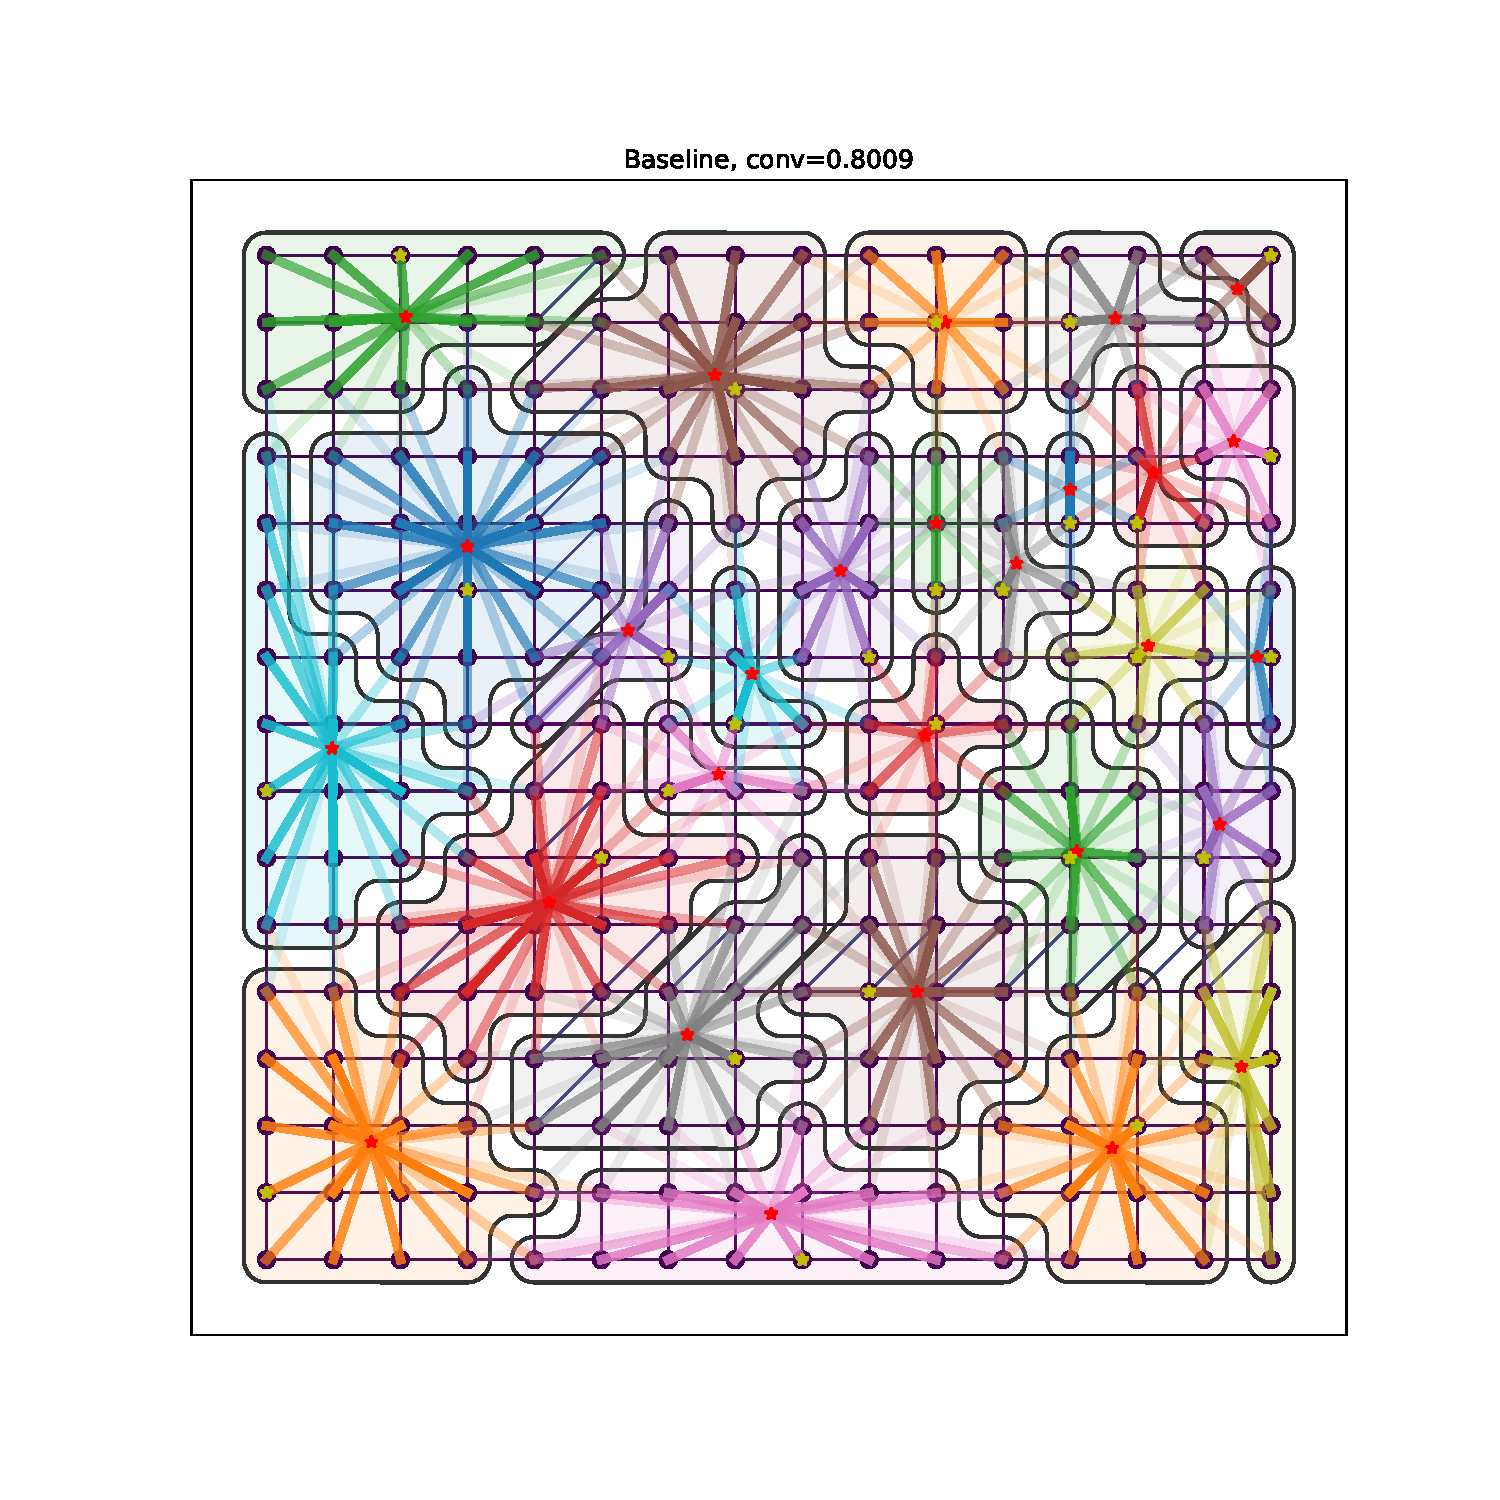
\includegraphics[width=\textwidth]{baseline.pdf}
    \caption{Lloyd Aggregates}
  \end{subfigure}
  \hfill
  \begin{subfigure}[t]{0.49\textwidth}
    \centering
    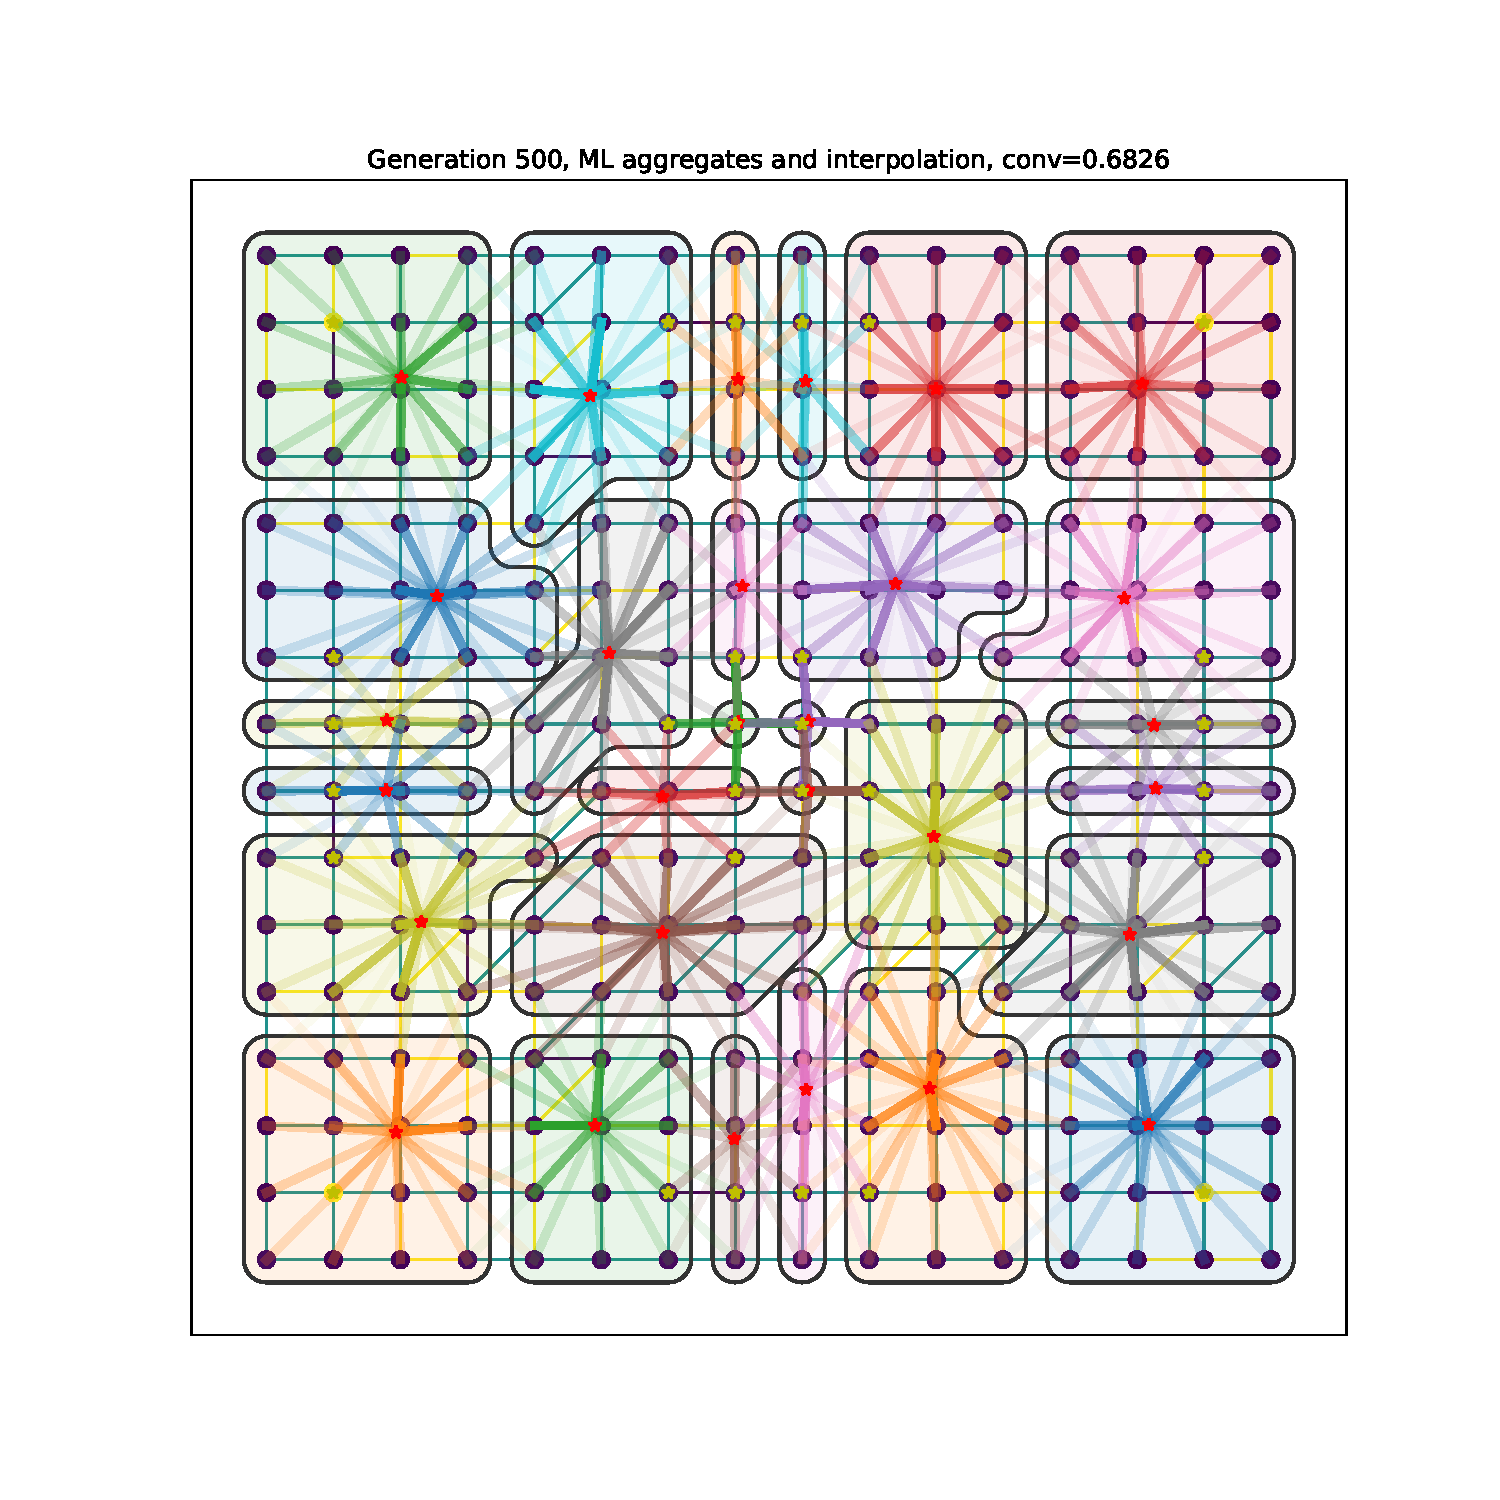
\includegraphics[width=\textwidth]{full.pdf}
    \caption{ML aggregates and interpolation, both networks trained concurrently}
  \end{subfigure}
    \caption{Aggregates for isotropic 2D Poisson, $16 \times 16$ grid.}
\end{figure}
\begin{figure}[h]
  \centering
  \begin{subfigure}[t]{0.49\textwidth}
    \centering
    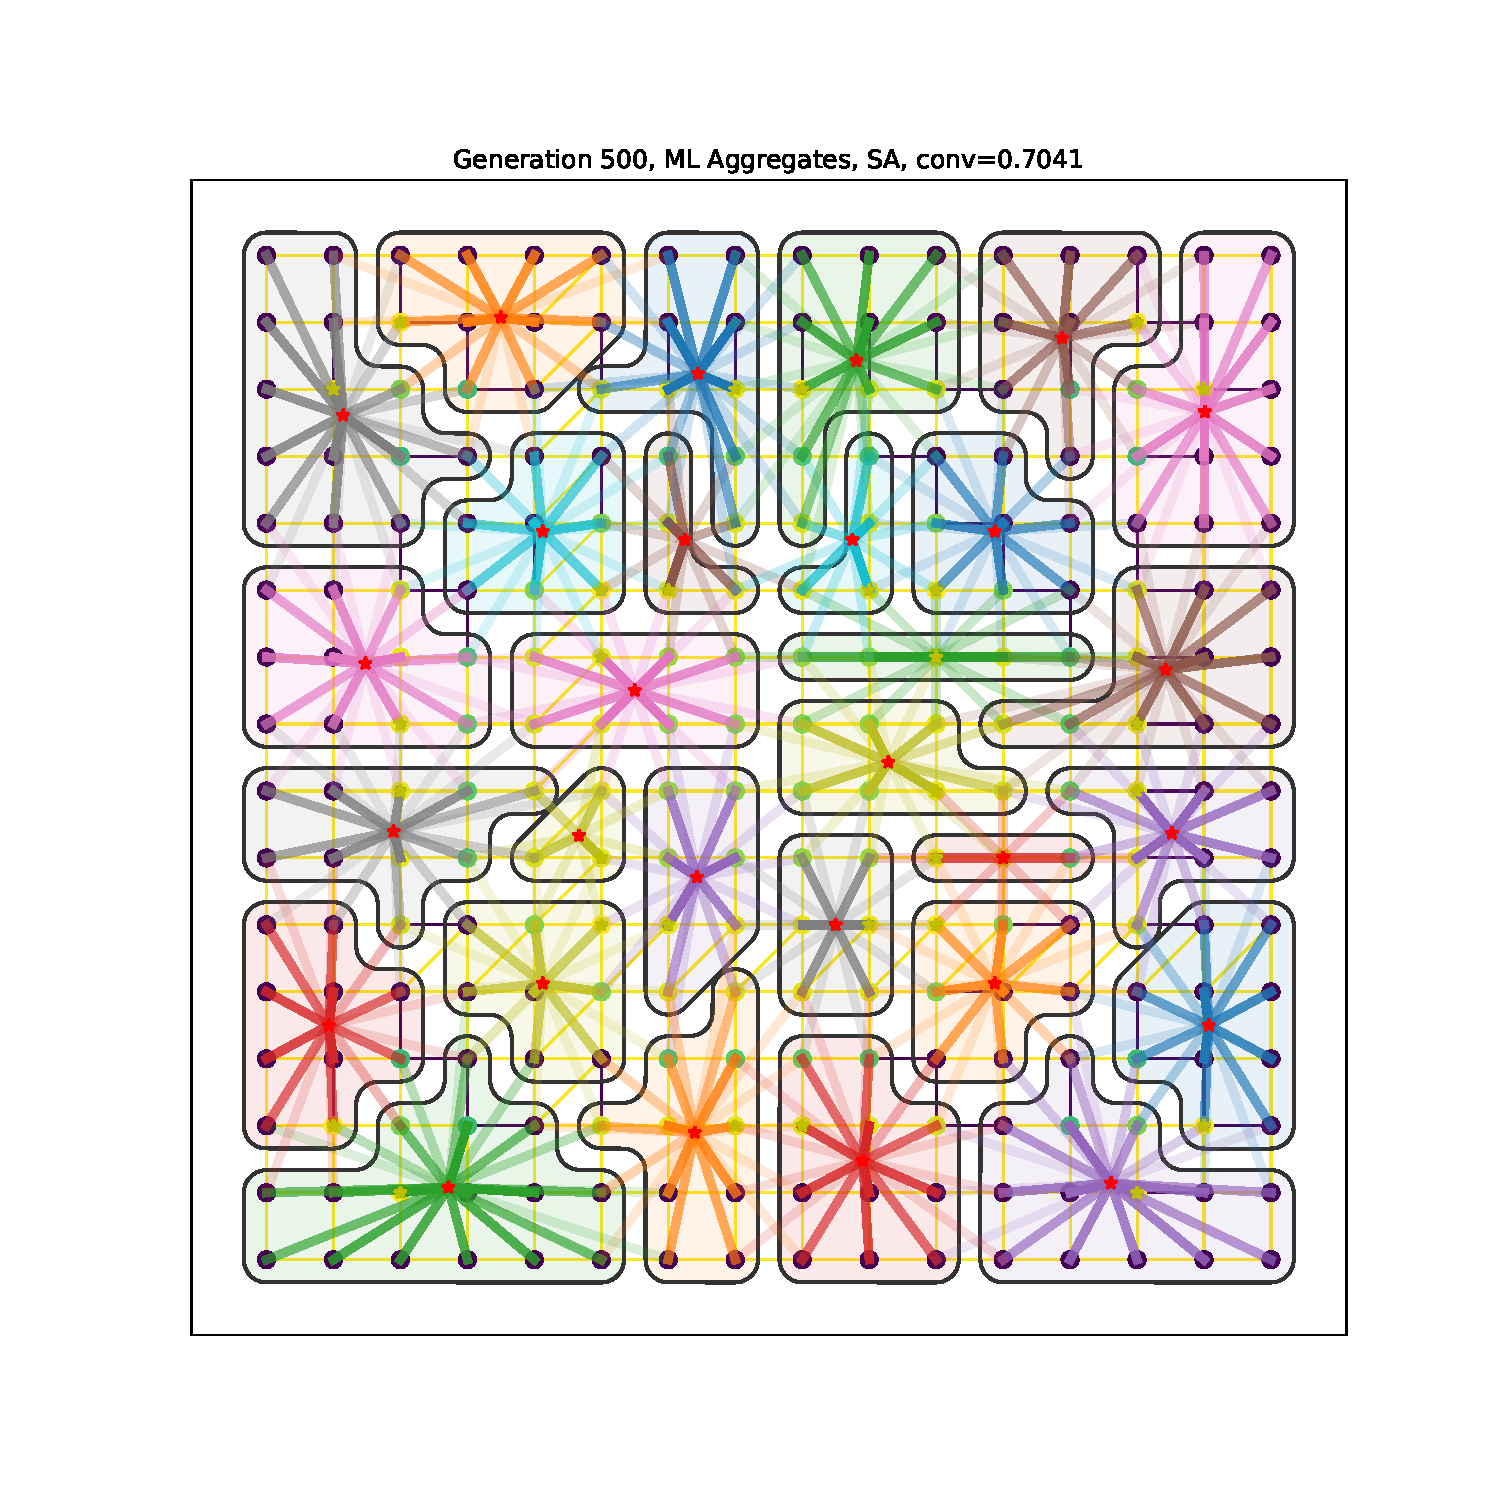
\includegraphics[width=\textwidth]{agg.pdf}
    \caption{ML aggregates with smoothed aggregation}
  \end{subfigure}
    \begin{subfigure}[t]{0.49\textwidth}
    \centering
    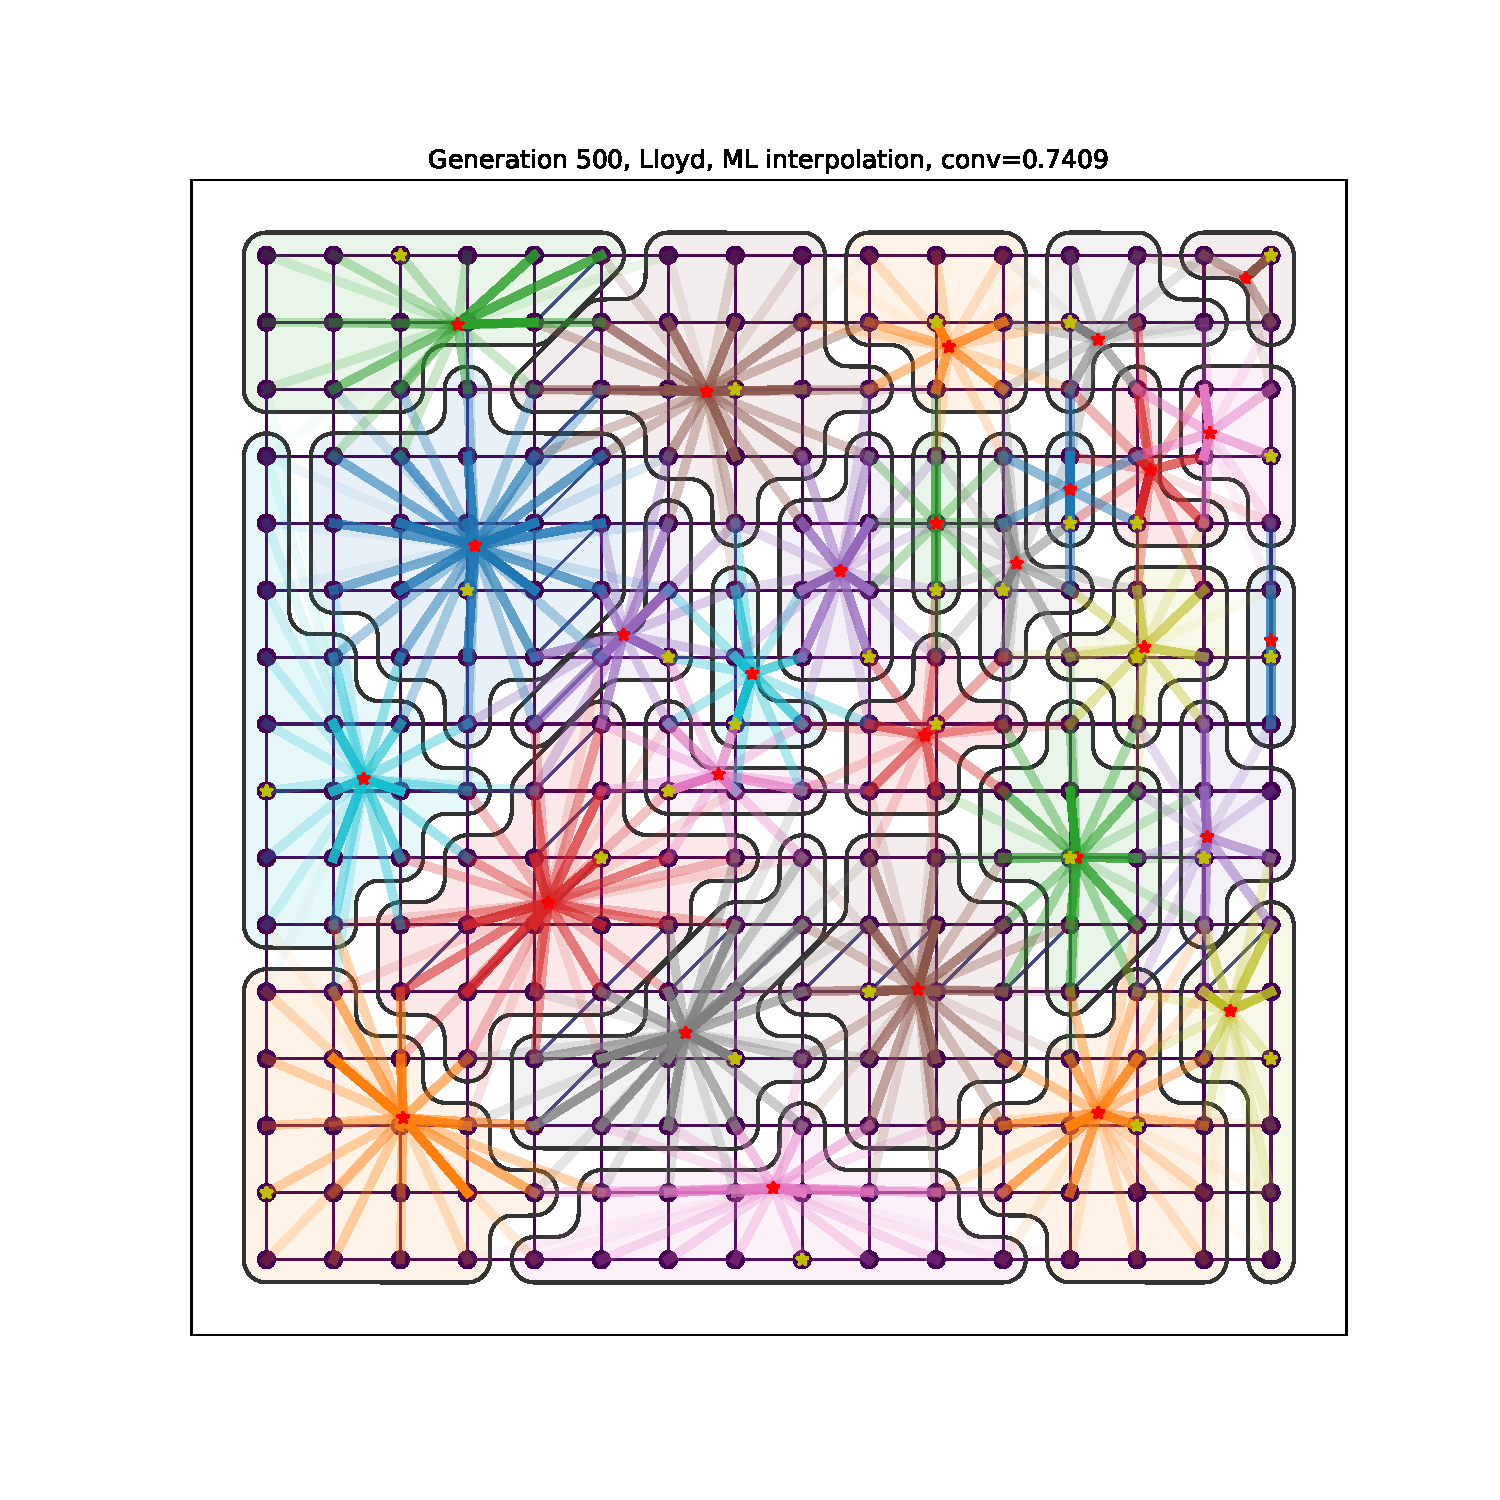
\includegraphics[width=\textwidth]{interp.pdf}
    \caption{Lloyd aggregates with ML interpolation}
    \end{subfigure}
    \begin{subfigure}[t]{0.49\textwidth}
    \centering
    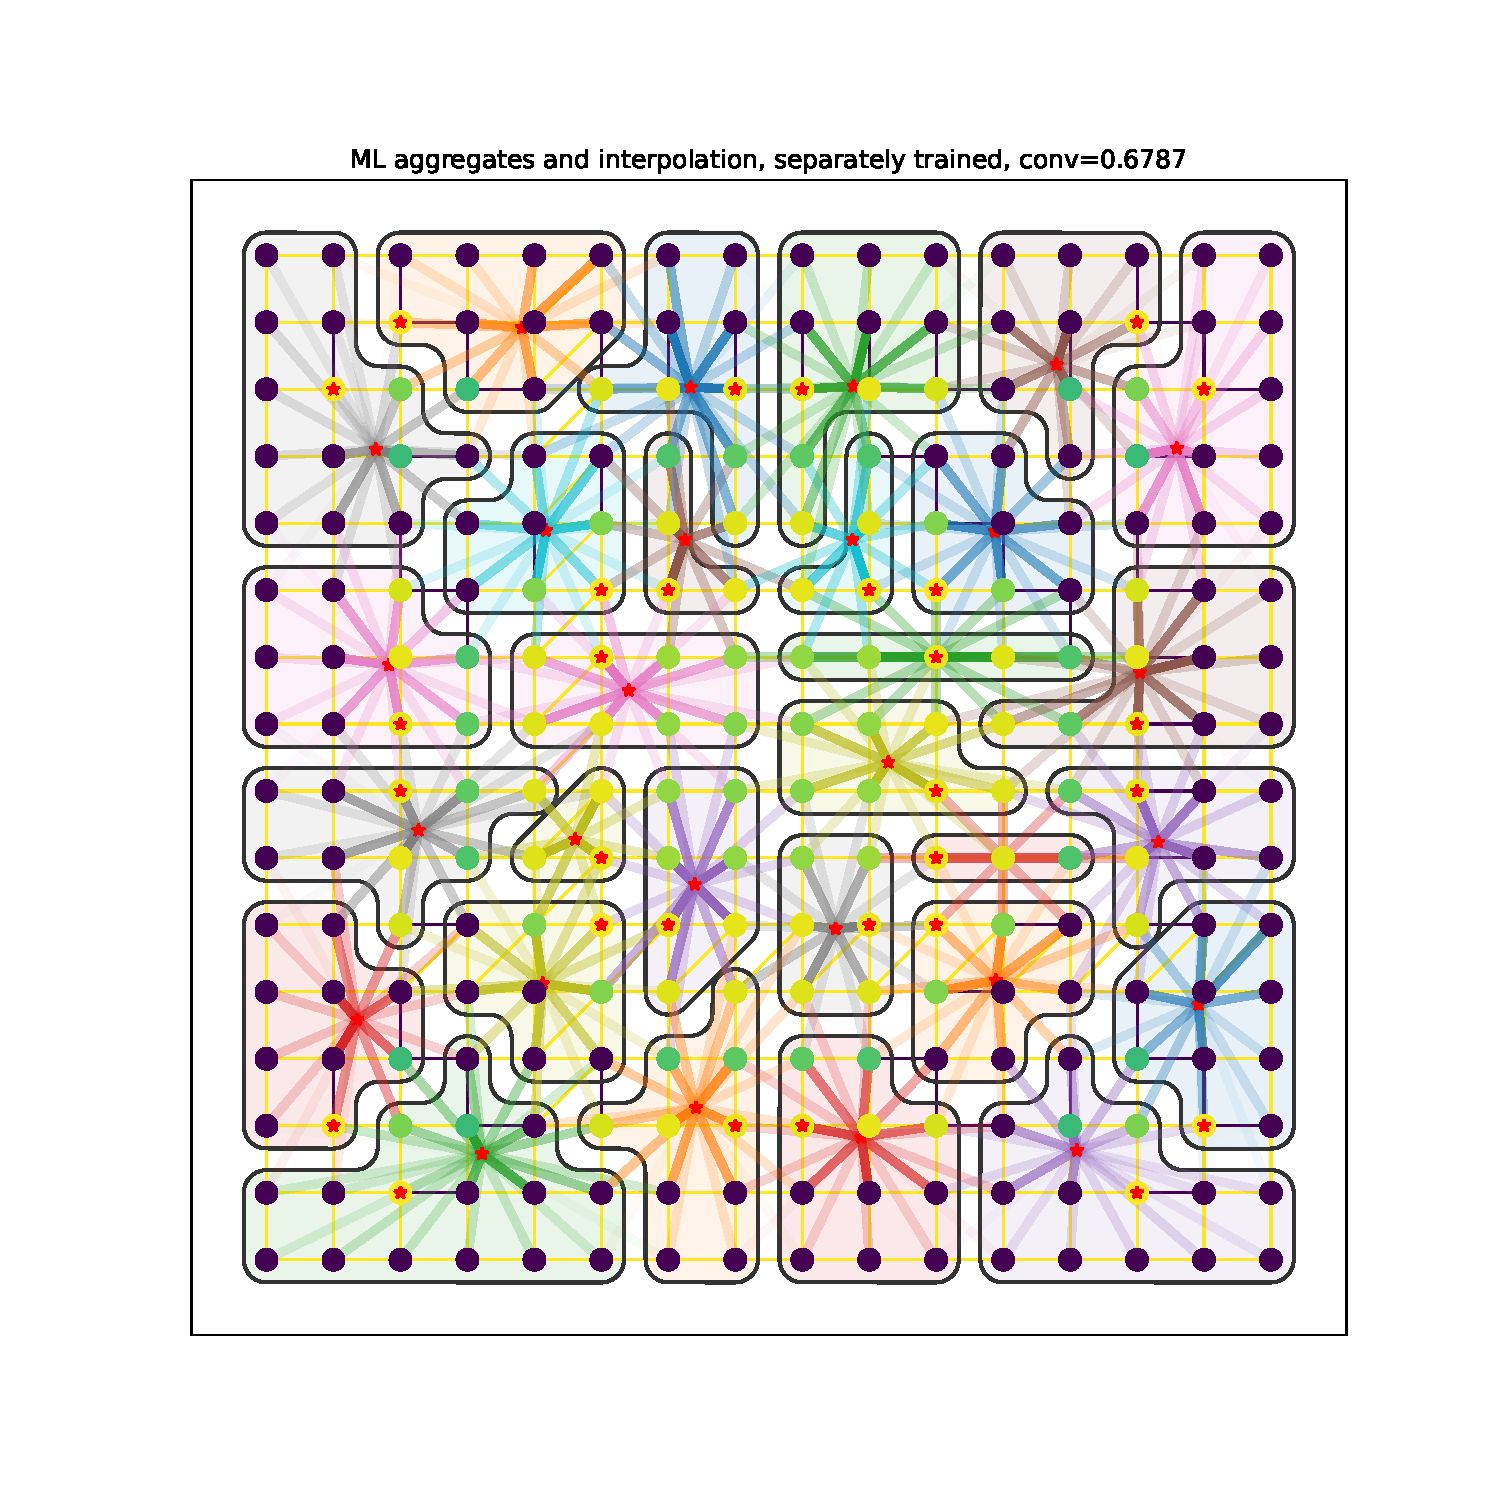
\includegraphics[width=\textwidth]{ablation.pdf}
  \end{subfigure}
  \caption{Aggregates for isotropic 2D Poisson, $16 \times 16$ grid, individual aggregation and interpolation networks separately trained then combined.}
  \label{fig:2d_isotropic}
\end{figure}
%% \begin{figure}[h]
%%   \centering
%%   \caption{Aggregates for isotropic 2D Poisson, $16 \times 16$ grid, individual aggregation and interpolation networks separately trained then combined.}
%%   \label{fig:2d_isotropic}
%% \end{figure}

\begin{table}[h]
  \centering
  \begin{tabular}{|c|c|c|c|}
    \hline
    Training Method & Full ML & Lloyd + ML Interpolation & ML Aggregates + SA \\
    \hline
    Concurrently & 0.68260 & 0.79306 & 0.77864 \\
    Separately & 0.67783 & 0.77547 & 0.72084 \\
    \hline
  \end{tabular}
  \caption{Convergence factors when swapping out different parts of the method.  The row for ``concurrently'' is when both networks are trained together to optimize convergence, while networks in ``separately'' are trained with either with Lloyd clustering or SA.}
\end{table}

\end{document}
